\documentclass[a4paper,10pt]{article}

\usepackage[utf8]{inputenc}
\usepackage[T1]{fontenc}
\usepackage[scaled=0.94]{helvet}
\renewcommand{\familydefault}{\sfdefault}
\usepackage{lmodern}
\usepackage{microtype}
\usepackage[a4paper,top=11mm,bottom=14mm,left=12.5mm,right=12.5mm,footskip=6.5mm]{geometry}
\usepackage[table]{xcolor}
\usepackage{tabularx}
\usepackage{booktabs}
\usepackage{array}
\usepackage{colortbl}
\usepackage{enumitem}
\usepackage{fancyhdr}
\usepackage{lastpage}
\usepackage{listings}
\usepackage{seqsplit}
\usepackage[skins]{tcolorbox}
\usepackage{tikz}
\usetikzlibrary{arrows.meta,positioning,shapes.geometric}
\usepackage[hidelinks]{hyperref}

% Paleta institucional (azul marinho academico + ardosia)
\definecolor{navy}{HTML}{0F3D75}
\definecolor{blueaccent}{HTML}{1D4ED8}
\definecolor{tealaccent}{HTML}{0F766E}
\definecolor{purpleaccent}{HTML}{5B21B6}
\definecolor{slate900}{HTML}{0F172A}
\definecolor{slate700}{HTML}{334155}
\definecolor{slate500}{HTML}{64748B}
\definecolor{rowalt}{HTML}{F8FAFC}
\definecolor{cardbg}{HTML}{F8FAFC}
\definecolor{bordergray}{HTML}{CBD5E1}
\definecolor{okbg}{HTML}{DCFCE7}
\definecolor{okfg}{HTML}{166534}
\definecolor{infobg}{HTML}{F0F9FF}
\definecolor{infoborder}{HTML}{0284C7}
\definecolor{warnbg}{HTML}{FEFCE8}
\definecolor{warnborder}{HTML}{CA8A04}
\definecolor{darkcodebg}{HTML}{0F172A}
\definecolor{darkcodefg}{HTML}{E2E8F0}
\definecolor{lightcodebg}{HTML}{F8FAFC}

% Rodape e cabecalho de pagina
\pagestyle{fancy}
\fancyhf{}
\renewcommand{\headrulewidth}{0pt}
\renewcommand{\footrulewidth}{0.4pt}
\renewcommand{\footrule}{\hbox to\headwidth{\color{bordergray}\leaders\hrule height \footrulewidth\hfill}}
\fancyfoot[L]{\fontsize{6.8}{8}\selectfont\color{slate500}UNOESC \textbullet{} 33506 Cyber Security — Avaliação A1/3}
\fancyfoot[R]{\fontsize{6.8}{8}\selectfont\color{slate500}Pedro Diniz; Luiz Felipe Kauê da Silva; Domingos Chicanha Fonseca; Wesley Warken — Página \thepage\ de \pageref{LastPage}}

% Configuracao global de paragrafos e listas
\setlength{\parindent}{0pt}
\setlength{\parskip}{3pt}
\setlist[itemize]{leftmargin=12pt,itemsep=1.2pt,topsep=1.5pt,parsep=0pt}
\renewcommand{\arraystretch}{1.18}

% Helpers tipograficos
\newcommand{\secbanner}[2]{%
  \vspace{4pt}%
  {\noindent\colorbox{navy}{\strut\hspace{2pt}\textcolor{white}{\bfseries\fontsize{7.5}{8.5}\selectfont #1}\hspace{2pt}}\hspace{5pt}%
  {\fontsize{9.8}{11}\selectfont\bfseries\color{navy}#2}}%
  \par\vspace{-3.5pt}{\color{blueaccent!25}\rule{\linewidth}{1pt}}\par\vspace{2.5pt}%
}
\newcommand{\subsec}[1]{%
  \vspace{3.5pt}{\noindent\fontsize{8.3}{9.5}\selectfont\bfseries\color{slate900}#1}\par\vspace{1.5pt}%
}
\newcommand{\code}[1]{%
  {\ttfamily\fontsize{7.0}{8.1}\selectfont\color{slate900}#1}%
}
\newcommand{\bcode}[1]{%
  {\ttfamily\fontsize{6.85}{8.0}\selectfont\color{slate900}\seqsplit{#1}}%
}
\newcommand{\okbadge}{%
  \colorbox{okbg}{\textcolor{okfg}{\bfseries\fontsize{6.5}{7.5}\selectfont OK}}%
}
\newcolumntype{L}[1]{>{\raggedright\arraybackslash}p{#1}}
\newcolumntype{C}[1]{>{\centering\arraybackslash}p{#1}}
\newcolumntype{Y}{>{\raggedright\arraybackslash}X}

% Listings com quebra automatica de linha e suporte UTF-8
\lstset{
  basicstyle=\ttfamily\fontsize{6.5}{7.7}\selectfont,
  breaklines=true,
  breakatwhitespace=false,
  postbreak={},
  escapeinside={(*@}{@*)},
  columns=fullflexible,
  keepspaces=true,
  showstringspaces=false,
  aboveskip=2.5pt,
  belowskip=3.5pt,
  xleftmargin=3pt,
  xrightmargin=3pt,
  framesep=3.5pt,
  framerule=0.5pt,
  literate=
    {á}{{\'a}}1 {à}{{\`a}}1 {â}{{\^a}}1 {ã}{{\~a}}1
    {é}{{\'e}}1 {ê}{{\^e}}1 {í}{{\'i}}1 {ó}{{\'o}}1
    {ô}{{\^o}}1 {õ}{{\~o}}1 {ú}{{\'u}}1 {ç}{{\c{c}}}1
    {Á}{{\'A}}1 {É}{{\'E}}1 {Í}{{\'I}}1 {Ó}{{\'O}}1
    {Ú}{{\'U}}1 {Ç}{{\c{C}}}1 {→}{{->}}2 {—}{{---}}1
    {–}{{--}}1 {≤}{{<=}}2
}
\lstdefinestyle{darkcode}{
  backgroundcolor=\color{darkcodebg},
  basicstyle=\ttfamily\fontsize{6.4}{7.6}\selectfont\color{darkcodefg},
  frame=single,
  rulecolor=\color{darkcodebg}
}
\lstdefinestyle{lightcode}{
  backgroundcolor=\color{lightcodebg},
  basicstyle=\ttfamily\fontsize{6.3}{7.4}\selectfont\color{slate900},
  frame=single,
  rulecolor=\color{bordergray}
}

% Caixas tcolorbox reutilizaveis
\tcbset{
  cardbox/.style={
    colback=cardbg,
    colframe=bordergray,
    boxrule=0.5pt,
    arc=2.5pt,
    left=5pt,right=5pt,top=4pt,bottom=4pt,
    boxsep=0pt
  },
  infobox/.style={
    colback=infobg,
    colframe=bordergray,
    borderline west={2.5pt}{0pt}{infoborder},
    boxrule=0.4pt,
    arc=2pt,
    left=7pt,right=6pt,top=4pt,bottom=4pt,
    boxsep=0pt
  },
  warnbox/.style={
    colback=warnbg,
    colframe=warnborder!45,
    borderline west={2.5pt}{0pt}{warnborder},
    boxrule=0.4pt,
    arc=2pt,
    left=7pt,right=6pt,top=4.5pt,bottom=4.5pt,
    boxsep=0pt
  },
  darkbox/.style={
    colback=darkcodebg,
    colframe=darkcodebg,
    colupper=darkcodefg,
    boxrule=0.4pt,
    arc=2.5pt,
    left=5.5pt,right=5.5pt,top=4pt,bottom=4pt,
    boxsep=0pt,
    before skip=2.5pt,
    after skip=3.5pt
  }
}

\begin{document}

% ==============================================================================
% PÁGINA 1: CABEÇALHO, ARQUITETURA, DIAGRAMA TIKZ E TABELA DE USUÁRIOS
% ==============================================================================
\noindent
\begin{minipage}[b]{0.57\linewidth}
  {\fontsize{7.2}{8.5}\selectfont\bfseries\color{navy}UNIVERSIDADE DO OESTE DE SANTA CATARINA (UNOESC) — ENGENHARIA DE COMPUTAÇÃO}\par
  \vspace{2pt}
  {\fontsize{13}{14.5}\selectfont\bfseries\color{slate900}Autenticação e Autorização — OAuth 2.0 + OpenID Connect}\par
  \vspace{1.5pt}
  {\fontsize{7.9}{9.2}\selectfont\color{slate700}Avaliação A1/3 — Disciplina 33506 (Cyber Security) \textbullet{} Opção 1: OpenID Provider Próprio + Aplicação Cliente}
\end{minipage}\hfill
\begin{minipage}[b]{0.41\linewidth}
  \begin{tcolorbox}[colback=cardbg,colframe=bordergray,borderline west={2.5pt}{0pt}{navy},boxrule=0.4pt,arc=2pt,left=6pt,right=5pt,top=3.5pt,bottom=3.5pt,boxsep=0pt]
    \fontsize{7.2}{9.2}\selectfont
    \textbf{Professor:} Odemir Moreira da Mata Junior\\
    \textbf{Acadêmicos:} Pedro Diniz; Luiz Felipe Kauê da Silva; Domingos Chicanha Fonseca; Wesley Warken\\
    \textbf{Data:} 26/11/2026 \quad|\quad \textbf{Stack:} Python 3.12, Flask, SQLite
  \end{tcolorbox}
\end{minipage}
\vspace{2pt}
{\color{navy}\rule{\linewidth}{1.6pt}}

\secbanner{1}{Arquitetura e Componentes Implementados}
{\fontsize{7.9}{9.8}\selectfont
O sistema implementa a \textbf{Opção 1} em dois processos independentes em Python (Flask + SQLite), com renderização 100\% no servidor — sem JavaScript no back-end e sem exposição de tokens em \code{localStorage} ou scripts do navegador. As credenciais do usuário trafegam exclusivamente entre o navegador e o Servidor de Autorização (OpenID Provider).
}

\vspace{2pt}
\noindent
\begin{minipage}[t]{0.492\linewidth}
  \begin{tcolorbox}[cardbox,height=32.5mm]
    {\fontsize{7.8}{9}\selectfont\bfseries\color{navy}Servidor de Autorização — \code{auth\_server/} (OP)}\\[-1pt]
    {\fontsize{6.9}{8}\selectfont\color{slate500}Portas: \code{:8443} (HTTPS) / \code{:8001} (HTTP local dev)}
    \begin{itemize}\fontsize{7.15}{8.6}\selectfont
      \item \code{GET /.well-known/openid-configuration} e \code{GET /jwks.json} (RSA com \code{kid} e rotação).
      \item \code{GET/POST /authorize}: \code{redirect\_uri} exata, login Argon2id, rate limit, consentimento e \code{code} (TTL $\le$ 60s).
      \item \code{POST /token}: \code{client\_secret\_post/basic}, PKCE S256, uso único + revogação em replay, RS256 e \code{no-store}.
      \item \code{GET/POST /userinfo} (Bearer) e \code{POST /logout}.
    \end{itemize}
  \end{tcolorbox}
\end{minipage}\hfill
\begin{minipage}[t]{0.492\linewidth}
  \begin{tcolorbox}[cardbox,height=32.5mm]
    {\fontsize{7.8}{9}\selectfont\bfseries\color{navy}Aplicação Cliente — \code{app/} (Relying Party)}\\[-1pt]
    {\fontsize{6.9}{8}\selectfont\color{slate500}Portas: \code{:8444} (HTTPS) / \code{:8000} (HTTP local dev)}
    \begin{itemize}\fontsize{7.15}{8.6}\selectfont
      \item \code{GET /}: status da sessão, decomposição do ID Token e checklist 10/10.
      \item \code{GET /login}: gera \code{state}, \code{nonce} e \code{code\_verifier} (256 bits) + \code{code\_challenge} S256.
      \item \code{GET /callback}: valida \code{state} antes de \code{/token} (sem retry), valida ID Token (\code{RS256}), chama \code{/userinfo} e vincula \code{(iss, sub)}.
      \item \code{GET /admin} (\code{admin}$\to$200; \code{user}$\to$403) e \code{POST /logout} (CSRF).
    \end{itemize}
  \end{tcolorbox}
\end{minipage}

\secbanner{2}{Diagrama do Fluxo Implementado (Authorization Code + PKCE S256 + OIDC)}
\begin{center}
\vspace{-2pt}
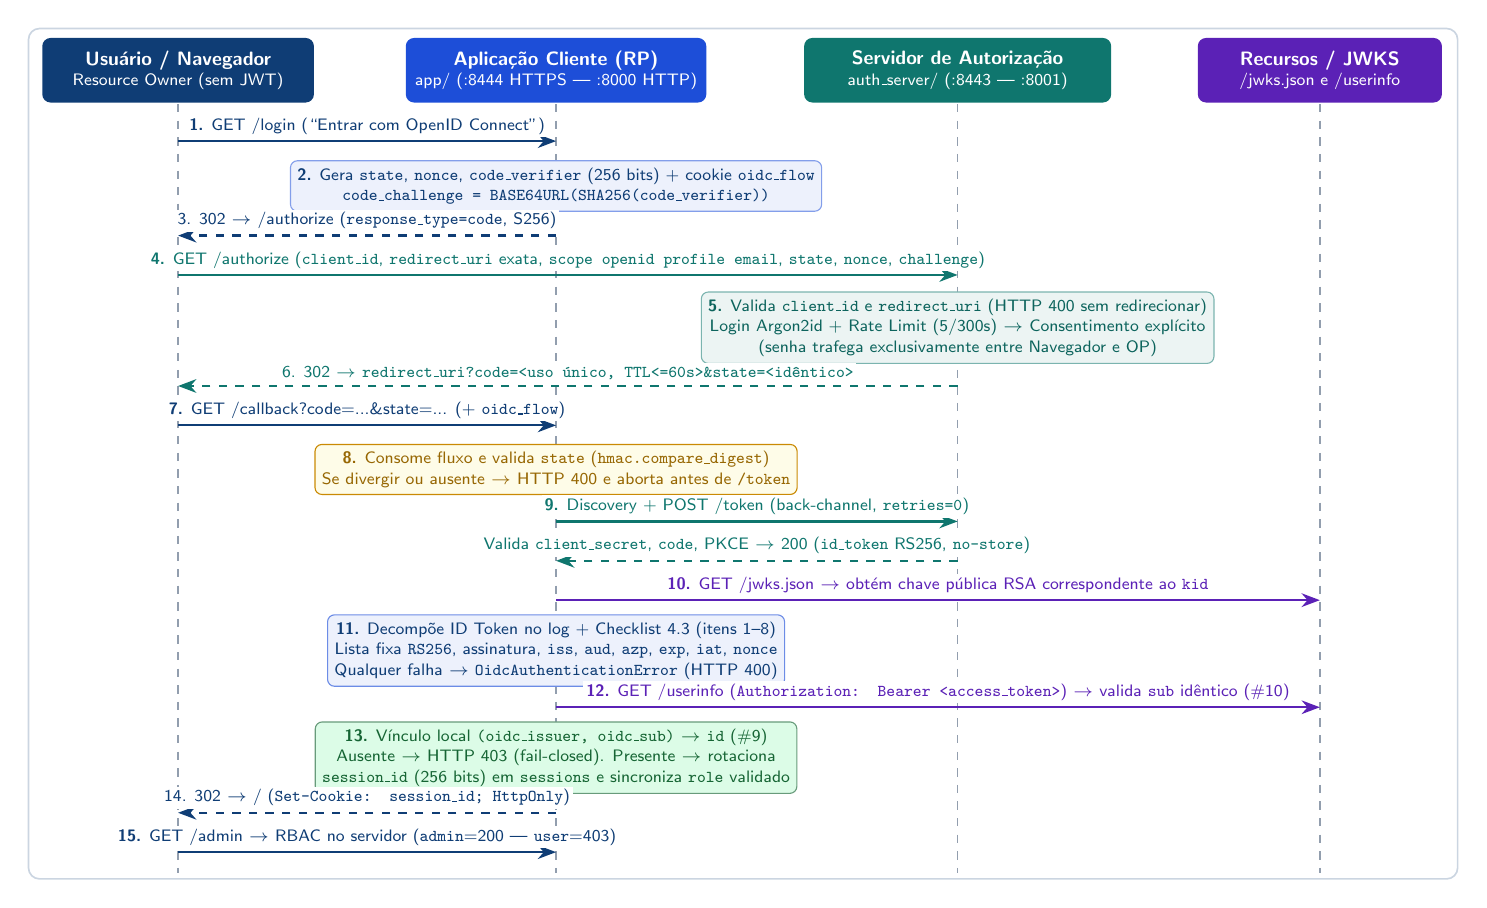
\begin{tikzpicture}[
  x=1cm, y=-1cm,
  >=Stealth,
  actor/.style={rectangle, rounded corners=3pt, minimum width=3.45cm, minimum height=0.82cm, align=center, text=white, font=\bfseries\fontsize{7.4}{8.5}\selectfont},
  note/.style={rectangle, rounded corners=2.5pt, draw, align=center, font=\fontsize{6.3}{7.4}\selectfont, inner sep=2.5pt},
  msg/.style={font=\fontsize{6.4}{7.2}\selectfont, fill=white, inner sep=1pt},
  arrB/.style={->, thick, color=navy},
  arrBD/.style={->, thick, dashed, color=navy},
  arrG/.style={->, thick, color=tealaccent},
  arrGD/.style={->, thick, dashed, color=tealaccent},
  arrP/.style={->, thick, color=purpleaccent}
]
  % Posicoes horizontais dos 4 atores (largura total ~18.0cm)
  \def\xU{1.8}
  \def\xRP{6.6}
  \def\xOP{11.7}
  \def\xRS{16.3}

  % Caixas dos atores
  \node[actor, fill=navy] (U) at (\xU, 0.45) {Usuário / Navegador\\[-1pt]{\normalfont\fontsize{6.1}{7}\selectfont\color{white!85}Resource Owner (sem JWT)}};
  \node[actor, fill=blueaccent, minimum width=3.8cm] (RP) at (\xRP, 0.45) {Aplicação Cliente (RP)\\[-1pt]{\normalfont\fontsize{6.1}{7}\selectfont\color{white!85}app/ (:8444 HTTPS | :8000 HTTP)}};
  \node[actor, fill=tealaccent, minimum width=3.9cm] (OP) at (\xOP, 0.45) {Servidor de Autorização\\[-1pt]{\normalfont\fontsize{6.1}{7}\selectfont\color{white!85}auth\_server/ (:8443 | :8001)}};
  \node[actor, fill=purpleaccent, minimum width=3.1cm] (RS) at (\xRS, 0.45) {Recursos / JWKS\\[-1pt]{\normalfont\fontsize{6.1}{7}\selectfont\color{white!85}/jwks.json e /userinfo}};

  % Linhas de vida
  \draw[dashed, color=slate500!70, line width=0.6pt] (\xU, 0.88) -- (\xU, 10.65);
  \draw[dashed, color=slate500!70, line width=0.6pt] (\xRP, 0.88) -- (\xRP, 10.65);
  \draw[dashed, color=slate500!70, line width=0.6pt] (\xOP, 0.88) -- (\xOP, 10.65);
  \draw[dashed, color=slate500!70, line width=0.6pt] (\xRS, 0.88) -- (\xRS, 10.65);

  % 1. GET /login
  \draw[arrB] (\xU, 1.35) -- node[msg, above=1pt] {\textbf{1.} GET /login (``Entrar com OpenID Connect'')} (\xRP, 1.35);

  % 2. Gera state, nonce, PKCE
  \node[note, fill=blueaccent!8, draw=blueaccent!55, text=navy, minimum width=5.3cm] at (\xRP, 1.92) {
    \textbf{2.} Gera \texttt{state}, \texttt{nonce}, \texttt{code\_verifier} (256 bits) + cookie \texttt{oidc\_flow}\\
    \texttt{code\_challenge = BASE64URL(SHA256(code\_verifier))}
  };

  % 3. 302 -> /authorize
  \draw[arrBD] (\xRP, 2.55) -- node[msg, above=1pt] {3. 302 $\to$ /authorize (\texttt{response\_type=code}, S256)} (\xU, 2.55);

  % 4. GET /authorize
  \draw[arrG] (\xU, 3.05) -- node[msg, above=1pt, text=tealaccent] {\textbf{4.} GET /authorize (\texttt{client\_id}, \texttt{redirect\_uri} exata, \texttt{scope openid profile email}, \texttt{state}, \texttt{nonce}, \texttt{challenge})} (\xOP, 3.05);

  % 5. OP valida, login e consentimento
  \node[note, fill=tealaccent!8, draw=tealaccent!55, text=tealaccent!85!black, minimum width=5.6cm] at (\xOP, 3.72) {
    \textbf{5.} Valida \texttt{client\_id} e \texttt{redirect\_uri} (HTTP 400 sem redirecionar)\\
    Login Argon2id + Rate Limit (5/300s) $\to$ Consentimento explícito\\
    (senha trafega exclusivamente entre Navegador e OP)
  };

  % 6. 302 -> redirect_uri
  \draw[arrGD] (\xOP, 4.46) -- node[msg, above=1pt, text=tealaccent] {6. 302 $\to$ \texttt{redirect\_uri?code=<uso único, TTL<=60s>\&state=<idêntico>}} (\xU, 4.46);

  % 7. GET /callback
  \draw[arrB] (\xU, 4.96) -- node[msg, above=1pt] {\textbf{7.} GET /callback?code=...\&state=... (+ \texttt{oidc\_flow})} (\xRP, 4.96);

  % 8. Valida state
  \node[note, fill=warnbg, draw=warnborder, text=warnborder!75!black, minimum width=5.1cm] at (\xRP, 5.52) {
    \textbf{8.} Consome fluxo e valida \texttt{state} (\texttt{hmac.compare\_digest})\\
    Se divergir ou ausente $\to$ HTTP 400 e aborta antes de \texttt{/token}
  };

  % 9. Discovery + POST /token
  \draw[arrG] (\xRP, 6.18) -- node[msg, above=1pt] {\textbf{9.} Discovery + POST /token (back-channel, \texttt{retries=0})} (\xOP, 6.18);
  \draw[arrGD] (\xOP, 6.68) -- node[msg, above=1pt, text=tealaccent] {Valida \texttt{client\_secret}, \texttt{code}, PKCE $\to$ 200 (\texttt{id\_token} RS256, \texttt{no-store})} (\xRP, 6.68);

  % 10. GET /jwks.json
  \draw[arrP] (\xRP, 7.18) -- node[msg, above=1pt, text=purpleaccent] {\textbf{10.} GET /jwks.json $\to$ obtém chave pública RSA correspondente ao \texttt{kid}} (\xRS, 7.18);

  % 11. Decompoe + Checklist 1-8
  \node[note, fill=blueaccent!8, draw=blueaccent!65, text=navy, minimum width=5.4cm] at (\xRP, 7.82) {
    \textbf{11.} Decompõe ID Token no log + Checklist 4.3 (itens 1--8)\\
    Lista fixa \texttt{RS256}, assinatura, \texttt{iss}, \texttt{aud}, \texttt{azp}, \texttt{exp}, \texttt{iat}, \texttt{nonce}\\
    Qualquer falha $\to$ \texttt{OidcAuthenticationError} (HTTP 400)
  };

  % 12. GET /userinfo
  \draw[arrP] (\xRP, 8.54) -- node[msg, above=1pt, text=purpleaccent] {\textbf{12.} GET /userinfo (\texttt{Authorization: Bearer <access\_token>}) $\to$ valida \texttt{sub} idêntico (\#10)} (\xRS, 8.54);

  % 13. Vinculo local + sessao
  \node[note, fill=okbg, draw=okfg!65, text=okfg, minimum width=5.4cm] at (\xRP, 9.18) {
    \textbf{13.} Vínculo local \texttt{(oidc\_issuer, oidc\_sub)} $\to$ \texttt{id} (\#9)\\
    Ausente $\to$ HTTP 403 (fail-closed). Presente $\to$ rotaciona\\
    \texttt{session\_id} (256 bits) em \texttt{sessions} e sincroniza \texttt{role} validado
  };

  % 14. 302 -> /
  \draw[arrBD] (\xRP, 9.88) -- node[msg, above=1pt] {14. 302 $\to$ / (\texttt{Set-Cookie: session\_id; HttpOnly})} (\xU, 9.88);

  % 15. GET /admin
  \draw[arrB] (\xU, 10.38) -- node[msg, above=1pt] {\textbf{15.} GET /admin $\to$ RBAC no servidor (\texttt{admin}=200 | \texttt{user}=403)} (\xRP, 10.38);

  % Moldura externa sutil
  \draw[rounded corners=4pt, color=bordergray, line width=0.6pt] (-0.1, -0.08) rectangle (18.05, 10.72);
\end{tikzpicture}
\vspace{-4pt}
\end{center}

\subsec{Tabela Local de Usuários (Item 4.1 — \code{app/storage.py:16-25})}
{\fontsize{7.1}{8.5}\selectfont
\begin{tabularx}{\linewidth}{|L{2.9cm}|L{5.1cm}|Y|}
  \hline
  \rowcolor{navy}\textcolor{white}{\bfseries Coluna} & \textcolor{white}{\bfseries Tipo / Restrição} & \textcolor{white}{\bfseries Finalidade no Sistema} \\
  \hline
  \code{id} & \code{INTEGER PRIMARY KEY} & Identificador interno na aplicação; gravado em \code{sessions.user\_id}. \\
  \hline
  \rowcolor{rowalt}\code{user\_name} & \code{TEXT NOT NULL UNIQUE} & Nome de exibição do usuário (nunca usado como chave de vínculo OIDC). \\
  \hline
  \code{full\_name} & \code{TEXT NOT NULL} & Nome completo exibido na interface autenticada. \\
  \hline
  \rowcolor{rowalt}\code{oidc\_issuer} + \code{oidc\_sub} & \code{TEXT NOT NULL, UNIQUE (oidc\_issuer, oidc\_sub)} & Chave composta de vínculo com o OpenID Provider (OIDC Core \S5.7). \\
  \hline
  \code{role} & \code{TEXT CHECK (role IN ('user','admin'))} & Perfil de autorização revalidado no servidor em cada requisição a \code{/admin}. \\
  \hline
  \rowcolor{rowalt}\code{created\_at} & \code{TEXT DEFAULT CURRENT\_TIMESTAMP} & Timestamp de auditoria do registro local. \\
  \hline
\end{tabularx}
}

\newpage
% ==============================================================================
% PÁGINA 2: ID TOKEN REAL DECODIFICADO E LOGS DE EXECUÇÃO
% ==============================================================================
\secbanner{3}{ID Token Real Decodificado (Execução Real — 26/11/2026)}
{\fontsize{8}{10}\selectfont
As três partes do JWS compacto abaixo foram capturadas diretamente da execução real dos dois servidores Flask (\code{auth\_server} em \code{http://localhost:8001} e \code{app} em \code{http://localhost:8000}, com login do usuário \code{admin} às 19:00:24 em 26/11/2026). Nenhum dado foi fabricado; credenciais, senhas, \code{client\_secret} e chaves privadas não constam neste documento.
}

\vspace{2pt}
\noindent
\begin{minipage}[t]{0.44\linewidth}
  \subsec{3.1 Cabeçalho (Header — Base64URL decodificado)}
\begin{lstlisting}[style=darkcode]
{
  "alg": "RS256",
  "kid": "rsa-2026-11-bedae646",
  "typ": "JWT"
}
\end{lstlisting}
  \subsec{3.2 Chave Pública Correspondente (\code{GET /jwks.json})}
  \begin{tcolorbox}[darkbox]
    \ttfamily\fontsize{6.3}{7.5}\selectfont\raggedright
    \{\\
    \hspace*{0.8em}"keys": [\\
    \hspace*{1.6em}\{\\
    \hspace*{2.4em}"alg": "RS256",\\
    \hspace*{2.4em}"e": "AQAB",\\
    \hspace*{2.4em}"kid": "rsa-2026-11-bedae646",\\
    \hspace*{2.4em}"kty": "RSA",\\
    \hspace*{2.4em}"n": "\seqsplit{opx2q1EZrQgVd9dLMt5U8oGmTDD-o85p1gDoP6ITDnr0GR3rROlFDrTiTBSvX6T-BFbBAtf5bq0rUgGrttvTPhQ1Eqk6WatGzn4-BuCHTgVspmBY7uBfbLif0dV2gE8QLK0jVgitfgRqmVGovz\_qsyeXqG5CyEcmrxl1Q7952AdE7fZZlc5y5f0hMKnRvTMNKAhCewb3\_J\_98B7U4gO7caJdPpTtvAjPmqIO5kVb0BeFw1-br-g45AnUraciVXg0ZbWZiHSoqilUhrpkhbMePjhTMtXlo6wosbdLyeUzUeagQnbTliBZxZpavg2vHexNR5T81xh\_lYRWGDubSr8RUQ}",\\
    \hspace*{2.4em}"use": "sig"\\
    \hspace*{1.6em}\}\\
    \hspace*{0.8em}]\\
    \}
  \end{tcolorbox}
\end{minipage}\hfill
\begin{minipage}[t]{0.535\linewidth}
  \subsec{3.3 Payload (Claims Validados — Base64URL decodificado)}
\begin{lstlisting}[style=darkcode]
{
  "iss": "http://localhost:8001",
  "sub": "1000000001",
  "aud": "app-cybersecurity-33506",
  "exp": 1795731322,
  "iat": 1795730422,
  "nonce": "Vc-DJRfUhUYA0Rq-INGmSHFuH0vJtVK6m7i8llxO_EA",
  "azp": "app-cybersecurity-33506",
  "name": "Administrador (Demo)",
  "email": "admin@unoesc.local",
  "email_verified": true,
  "role": "admin"
}
\end{lstlisting}
  {\fontsize{7.2}{8.8}\selectfont\color{slate700}
  Observe \code{exp - iat = 1795731322 - 1795730422 = 900 s} (15 minutos), \code{iss} idêntico ao \code{issuer} da descoberta e todos os 11 claims exigidos na Seção 2.5 presentes.\par}
  \subsec{3.4 Resposta Real de \code{GET /userinfo} (Bearer Access Token)}
\begin{lstlisting}[style=darkcode]
{
  "sub": "1000000001",
  "name": "Administrador (Demo)",
  "email": "admin@unoesc.local",
  "email_verified": true
}
\end{lstlisting}
\end{minipage}

\subsec{3.5 Assinatura Digital (Signature — RS256 / RSA-2048, 256 bytes)}
\begin{tcolorbox}[darkbox]
  \ttfamily\fontsize{6.4}{7.7}\selectfont\raggedright
  Algoritmo: RSASSA-PKCS1-v1\_5 com SHA-256 (RS256) | Tamanho decodificado: 256 bytes (2048 bits)\\
  Entrada assinada: BASE64URL(header) + "." + BASE64URL(payload) | Chave de verificação: kid="rsa-2026-11-bedae646"\\[3pt]
  Base64URL (342 caracteres):\\
  \seqsplit{mR4hwLj8UvmGqv7yUnWP5Vx-lm4OkIwGXHkNyGnJXE3pQdzuK5MeXE70wSL1x3vHDhRs1O9iQ4lg9vIXrR1WGi1DgdAA3YajvnVoSQtFX25vkEXMyk2zHtYZ5j\_qjZj\_DxhQyFZ8JHYqbzwvi0p\_U\_9rOAkewNrHirzzAZ2c9lS\_3sWpdnbh7ebQTLtVjfT77xQiY1WoQ9X4UBOL9ZH391SYf8NeWl7DyzVdZi6Cs8qMnRi4JAR5SPLoXfUnACNyClkdvnMdy6MAwZ2BfeklBobLXFoi5OnqGRvx\_BBQ\_hrDHYB7-X3QP-iQYSOpg\_bI8BPkkd2yyjpWlbIEXLtkiA}\\[3pt]
  Hexadecimal (prefixo dos primeiros 32 bytes decodificados):\\
  \seqsplit{991e21c0b8fc52f986aafef252758fe55c7e966e0e908c065c790dc869c95c4d...}
\end{tcolorbox}

\subsec{3.6 Evidência de Execução Real nos Logs dos Servidores (Item 4.2.7 + Mascaramento de URLs)}
{\fontsize{7.8}{9.5}\selectfont
Durante a execução ponta a ponta, a Aplicação Cliente registra a decomposição do ID Token no log do servidor em nível \code{INFO} (\code{app/oidc.py:251-257}) e ambos os servidores mascaram query strings sensíveis (\code{/authorize?[REDACTED]} e \code{/callback?[REDACTED]}) para evitar vazamento de \code{code} e \code{state}:
}
\begin{lstlisting}[style=lightcode]
# Log real do Servidor de Autorizacao (auth_server, porta 8001)
127.0.0.1 - - [26/Nov/2026 19:00:11] "GET /authorize?[REDACTED] HTTP/1.1" 200 -
127.0.0.1 - - [26/Nov/2026 19:00:13] "POST /authorize HTTP/1.1" 200 -
127.0.0.1 - - [26/Nov/2026 19:00:16] "POST /authorize HTTP/1.1" 302 -
127.0.0.1 - - [26/Nov/2026 19:00:20] "GET /.well-known/openid-configuration HTTP/1.1" 200 -
127.0.0.1 - - [26/Nov/2026 19:00:22] "POST /token HTTP/1.1" 200 -
127.0.0.1 - - [26/Nov/2026 19:00:24] "GET /jwks.json HTTP/1.1" 200 -
127.0.0.1 - - [26/Nov/2026 19:00:26] "GET /userinfo HTTP/1.1" 200 -

# Log real da Aplicacao Cliente (app, porta 8000) -- login admin (200), logout (303->401) e login usuario (403)
127.0.0.1 - - [26/Nov/2026 19:00:09] "GET /login HTTP/1.1" 302 -
[2026-11-26 19:00:24,746] INFO in oidc: ID Token decomposto | header={"alg": "RS256", "kid": "rsa-2026-11-bedae646", "typ": "JWT"} | payload={"aud": "app-cybersecurity-33506", "azp": "app-cybersecurity-33506", "email": "admin@unoesc.local", "email_verified": true, "exp": 1795731322, "iat": 1795730422, "iss": "http://localhost:8001", "name": "Administrador (Demo)", "nonce": "Vc-DJRfUhUYA0Rq-INGmSHFuH0vJtVK6m7i8llxO_EA", "role": "admin", "sub": "1000000001"} | signature_bytes=256 signature_b64=mR4hwLj8UvmGqv7yUnWP5Vx-...
127.0.0.1 - - [26/Nov/2026 19:00:26] "GET /callback?[REDACTED] HTTP/1.1" 302 -
127.0.0.1 - - [26/Nov/2026 19:00:30] "GET /admin HTTP/1.1" 200 -
127.0.0.1 - - [26/Nov/2026 19:00:32] "POST /logout HTTP/1.1" 303 -
127.0.0.1 - - [26/Nov/2026 19:00:35] "GET /admin HTTP/1.1" 401 -
[2026-11-26 19:00:52,358] INFO in oidc: ID Token decomposto | header={"alg": "RS256", "kid": "rsa-2026-11-bedae646", "typ": "JWT"} | payload={..., "role": "user", "sub": "1000000002"} | signature_bytes=256 signature_b64=RG4gHrko6TGpop6DcIzZTmt...
127.0.0.1 - - [26/Nov/2026 19:00:54] "GET /callback?[REDACTED] HTTP/1.1" 302 -
127.0.0.1 - - [26/Nov/2026 19:00:56] "GET /admin HTTP/1.1" 403 -
\end{lstlisting}

\begin{tcolorbox}[infobox]
  {\fontsize{7.5}{9.3}\selectfont
  \textbf{Cookie de sessão emitido no callback (execução real):} \code{session\_id=<43 chars / 256 bits aleatórios>; Max-Age=28800; HttpOnly; Path=/; SameSite=Lax} (acrescido de \code{Secure} quando servido em HTTPS, via \code{"secure": request.is\_secure} em \code{app/routes.py:16}), simultâneo ao descarte imediato do cookie temporário \code{oidc\_flow} (\code{Max-Age=0}).}
\end{tcolorbox}

\newpage
% ==============================================================================
% PÁGINA 3: CHECKLIST DO ITEM 4.3 (10/10 COM ARQUIVO:LINHA E EVIDÊNCIA REAL)
% ==============================================================================
\secbanner{4}{Checklist de Validação do ID Token (Item 4.3 — 10/10 Concluídos)}
{\fontsize{8}{9.8}\selectfont
Cada verificação exigida no item 4.3 do enunciado é executada no back-end da Aplicação Cliente antes da criação da sessão local. A tabela abaixo mapeia a referência normativa, a implementação exata (\code{arquivo:linha}) e a evidência real obtida no fluxo ao vivo e na suíte automatizada.
}

\vspace{2pt}
{\fontsize{7.15}{8.6}\selectfont
\renewcommand{\arraystretch}{1.24}
\begin{tabularx}{\linewidth}{|C{0.5cm}|L{4.5cm}|L{3.1cm}|C{0.9cm}|Y|}
  \hline
  \rowcolor{navy}\textcolor{white}{\bfseries \#} & \textcolor{white}{\bfseries Verificação e Referência} & \textcolor{white}{\bfseries Implementação (\texttt{arquivo:linha})} & \textcolor{white}{\bfseries Status} & \textcolor{white}{\bfseries Evidência Real (Fluxo ao Vivo e Testes)} \\
  \hline
  \textbf{1} & Assinatura conferida com chave pública do emissor por \code{kid}; chave não encontrada deve ser erro.\newline{\color{slate500}\fontsize{6.6}{7.6}\selectfont OIDC Core \S3.1.3.7 (6-7); RFC 8725 \S3.1} & \code{app/oidc.py:221-231}\newline\code{app/oidc.py:267-296} & \okbadge & Fluxo real: \bcode{kid=rsa-2026-11-bedae646} localizado em \code{/jwks.json} e verificado via RSA-2048.\newline Negativo: \bcode{test\_neg\_12} (\code{Signature verification failed}) e \bcode{test\_kid\_desconhecido...} (\code{Chave publica nao encontrada no JWKS}). \\
  \hline
  \rowcolor{rowalt}\textbf{2} & Algoritmo na lista fixa aceita; \code{alg="none"} é sempre rejeitado.\newline{\color{slate500}\fontsize{6.6}{7.6}\selectfont RFC 8725 \S2.1, \S3.1} & \code{app/oidc.py:20}\newline\code{app/oidc.py:262-264}\newline\code{app/oidc.py:284} & \okbadge & Constante fixa \bcode{ALLOWED\_ID\_TOKEN\_ALGORITHMS = ("RS256",)}. Fluxo real: \code{alg=RS256}.\newline Negativos: \bcode{test\_neg\_01} (\code{Algoritmo de ID Token rejeitado: 'none'.}) e \bcode{test\_neg\_02} (\code{rejeitado: 'HS256'.}). \\
  \hline
  \textbf{3} & \code{iss} idêntico ao \code{issuer} publicado na descoberta.\newline{\color{slate500}\fontsize{6.6}{7.6}\selectfont OIDC Core \S3.1.3.7 (2)} & \code{app/oidc.py:181-182}\newline\code{app/oidc.py:316-318} & \okbadge & Comparação \bcode{hmac.compare\_digest(iss, expected\_issuer)}. Fluxo real: \code{iss = "http://localhost:8001"}.\newline Negativo: \bcode{test\_neg\_04} (\code{Claim iss do ID Token diverge do emissor esperado.}). \\
  \hline
  \rowcolor{rowalt}\textbf{4} & \code{aud} contém o \code{client\_id} da aplicação.\newline{\color{slate500}\fontsize{6.6}{7.6}\selectfont OIDC Core \S3.1.3.7 (3)} & \code{app/oidc.py:329-338} & \okbadge & Aceita string ou lista de strings; exige \bcode{expected\_client\_id} em \code{aud\_list}. Fluxo real: \bcode{aud = "app-cybersecurity-33506"}.\newline Negativo: \bcode{test\_neg\_03} (\code{Claim aud do ID Token nao contem o client\_id da aplicacao.}). \\
  \hline
  \textbf{5} & Se \code{aud} tiver mais de um valor, \code{azp} é validado.\newline{\color{slate500}\fontsize{6.6}{7.6}\selectfont OIDC Core \S3.1.3.7 (4-5)} & \code{app/oidc.py:349-355} & \okbadge & Exige \code{azp == client\_id} quando \code{len(aud\_list) > 1} ou quando \code{azp} está presente. Fluxo real: \bcode{azp = "app-cybersecurity-33506"}.\newline Teste: \bcode{test\_azp\_com\_multiplos\_aud\_e\_mascara\_log\_callback} (\code{PASSED}). \\
  \hline
  \rowcolor{rowalt}\textbf{6} & \code{exp} está no futuro, com tolerância máxima de poucos minutos.\newline{\color{slate500}\fontsize{6.6}{7.6}\selectfont OIDC Core \S3.1.3.7 (9)} & \code{app/oidc.py:368-372}\newline\code{app/config.py:27} & \okbadge & Rejeita se \code{exp < now - 60} (skew máximo de 60s). Fluxo real: \code{exp=1795731322} (900s à frente).\newline Negativo: \bcode{test\_neg\_05} (\code{ID Token expirado (claim exp vencido).}). \\
  \hline
  \textbf{7} & \code{iat} não está no futuro.\newline{\color{slate500}\fontsize{6.6}{7.6}\selectfont OIDC Core \S3.1.3.7 (10)} & \code{app/oidc.py:383-387} & \okbadge & Rejeita se \code{iat > now + 60}. Fluxo real: \code{iat=1795730422}.\newline Negativo: \bcode{test\_neg\_06} (\code{Claim iat do ID Token esta no futuro.}). \\
  \hline
  \rowcolor{rowalt}\textbf{8} & \code{nonce} idêntico ao enviado na requisição.\newline{\color{slate500}\fontsize{6.6}{7.6}\selectfont OIDC Core \S3.1.3.7 (11)} & \code{app/oidc.py:398-400} & \okbadge & Comparação \bcode{hmac.compare\_digest(nonce, expected\_nonce)}. Fluxo real: \bcode{nonce=Vc-DJRfUhUYA0Rq-INGmSHFuH0vJtVK6m7i8llxO\_EA}.\newline Negativo: \bcode{test\_neg\_07} (\code{Claim nonce do ID Token diverge do valor enviado.}). \\
  \hline
  \textbf{9} & \code{sub} localizado na tabela e convertido no \code{id} interno.\newline{\color{slate500}\fontsize{6.6}{7.6}\selectfont OIDC Core \S5.7} & \code{app/storage.py:117-122}\newline\code{app/routes.py:121-139} & \okbadge & Consulta \code{WHERE oidc\_issuer = ? AND oidc\_sub = ?}. Fluxo real: \code{sub="1000000001"} $\to$ \code{id=1} (admin); \code{sub="1000000002"} $\to$ \code{id=2} (user).\newline Ausente $\to$ HTTP 403 (\bcode{test\_kid\_desconhecido\_sub\_nao\_cadastrado...}). \\
  \hline
  \rowcolor{rowalt}\textbf{10} & Se \code{/userinfo} for usado, o \code{sub} devolvido é igual ao do ID Token.\newline{\color{slate500}\fontsize{6.6}{7.6}\selectfont OIDC Core \S5.3.2} & \code{app/oidc.py:417-445}\newline\code{app/oidc.py:515-525} & \okbadge & Chamada obrigatória com \code{Authorization: Bearer <access\_token>}. Fluxo real: \code{userinfo["sub"] == "1000000001" == id\_token["sub"]}.\newline Divergente $\to$ rejeitado em \bcode{test\_kid\_desconhecido\_sub\_nao\_cadastrado...}. \\
  \hline
\end{tabularx}
}

\vspace{5pt}
\subsec{Verificações Complementares de Protocolo (Seções 2 e 4)}
\noindent
\begin{minipage}[t]{0.49\linewidth}
  \begin{tcolorbox}[cardbox]
    {\fontsize{7.7}{9}\selectfont\bfseries\color{navy}Descoberta, JWKS e Rotação de Chaves}\par\vspace{1.5pt}
    {\fontsize{7.3}{9}\selectfont\color{slate700}
    \bcode{test\_discovery\_jwks\_e\_rotacao\_de\_chave\_rsa} comprova que \bcode{/.well-known/openid-configuration} expõe todos os metadados do item 2.1 e que \bcode{KeyManager.rotate\_key()} (\code{auth\_server/keys.py:66-76}) adiciona nova chave ativa mantendo o \code{kid} anterior em \code{/jwks.json}, validando simultaneamente tokens antigos e novos durante a janela de transição.}
  \end{tcolorbox}
\end{minipage}\hfill
\begin{minipage}[t]{0.49\linewidth}
  \begin{tcolorbox}[cardbox]
    {\fontsize{7.7}{9}\selectfont\bfseries\color{navy}Sessão Local, Rotação e Erros no Callback}\par\vspace{1.5pt}
    {\fontsize{7.3}{9}\selectfont\color{slate700}
    \bcode{test\_implicit\_proibido\_callback\_access\_denied\_e\_rotacao\_sessao} comprova rejeição de \code{response\_type=token} (HTTP 400 sem redirecionar), tratamento amigável de \code{error=access\_denied} no callback (HTTP 400 sem criar sessão, item 4.6) e rotação obrigatória do \code{session\_id} no login invalidando o identificador anterior (item 4.4).}
  \end{tcolorbox}
\end{minipage}

\newpage
% ==============================================================================
% PÁGINA 4: TESTES NEGATIVOS OBRIGATÓRIOS — CASOS 1 A 9
% ==============================================================================
\secbanner{5}{Testes Negativos Obrigatórios (Item 5 — Casos 1 a 9)}
{\fontsize{8}{9.8}\selectfont
Todos os 15 cenários negativos obrigatórios da Seção 5 estão automatizados em \code{tests/test\_security\_suite.py} e foram executados sobre a implementação real. As colunas abaixo apresentam o resultado esperado, o teste correspondente e a saída real capturada na execução.
}

\vspace{2pt}
{\fontsize{7.15}{8.6}\selectfont
\renewcommand{\arraystretch}{1.28}
\begin{tabularx}{\linewidth}{|C{0.5cm}|L{3.9cm}|L{2.3cm}|L{3.9cm}|Y|}
  \hline
  \rowcolor{navy}\textcolor{white}{\bfseries \#} & \textcolor{white}{\bfseries Cenário de Ataque ou Falha} & \textcolor{white}{\bfseries Esperado} & \textcolor{white}{\bfseries Teste / Mecanismo} & \textcolor{white}{\bfseries Evidência Real de Execução (Exceção / HTTP / Log)} \\
  \hline
  \textbf{1} & ID Token com \code{alg="none"} (assinatura vazia) & Rejeitado & \bcode{test\_neg\_01\_id\_token\_alg\_none\_rejeitado}\newline\code{app/oidc.py:263} & \code{PASSED} — Exceção real:\newline\code{OidcAuthenticationError: Algoritmo de ID Token rejeitado: 'none'.} \\
  \hline
  \rowcolor{rowalt}\textbf{2} & ID Token reassinado em \code{HS256} usando a chave pública RSA (PEM) como segredo HMAC & Rejeitado & \bcode{test\_neg\_02\_id\_token\_reassinado\_hs256\_com\_chave\_publica\_rejeitado}\newline\code{app/oidc.py:20,263,284} & \code{PASSED} — Exceção real:\newline\code{OidcAuthenticationError: Algoritmo de ID Token rejeitado: 'HS256'.} \\
  \hline
  \textbf{3} & ID Token assinado validamente em RS256, mas com \code{aud="outro-client-id"} & Rejeitado & \bcode{test\_neg\_03\_id\_token\_aud\_outro\_client\_id\_rejeitado}\newline\code{app/oidc.py:337-338} & \code{PASSED} — Exceção real:\newline\code{OidcAuthenticationError: Claim aud do ID Token nao contem o client\_id da aplicacao.} \\
  \hline
  \rowcolor{rowalt}\textbf{4} & ID Token assinado validamente, mas com \bcode{iss="https://attacker.example"} & Rejeitado & \bcode{test\_neg\_04\_id\_token\_iss\_diferente\_rejeitado}\newline\code{app/oidc.py:317-318} & \code{PASSED} — Exceção real:\newline\code{OidcAuthenticationError: Claim iss do ID Token diverge do emissor esperado.} \\
  \hline
  \textbf{5} & ID Token com \code{exp} vencido (\code{now - 300s}, fora da tolerância de 60s) & Rejeitado & \bcode{test\_neg\_05\_id\_token\_exp\_vencido\_rejeitado}\newline\code{app/oidc.py:371-372} & \code{PASSED} — Exceção real:\newline\code{OidcAuthenticationError: ID Token expirado (claim exp vencido).} \\
  \hline
  \rowcolor{rowalt}\textbf{6} & ID Token com \code{iat} no futuro (\code{now + 600s}) & Rejeitado & \bcode{test\_neg\_06\_id\_token\_iat\_no\_futuro\_rejeitado}\newline\code{app/oidc.py:386-387} & \code{PASSED} — Exceção real:\newline\code{OidcAuthenticationError: Claim iat do ID Token esta no futuro.} \\
  \hline
  \textbf{7} & ID Token com \bcode{nonce="nonce-atacante-replay"} divergente do enviado & Rejeitado & \bcode{test\_neg\_07\_id\_token\_nonce\_diferente\_rejeitado}\newline\code{app/oidc.py:399-400} & \code{PASSED} — Exceção real:\newline\code{OidcAuthenticationError: Claim nonce do ID Token diverge do valor enviado.} \\
  \hline
  \rowcolor{rowalt}\textbf{8} & \code{GET /callback} com \code{state} divergente ou ausente & Fluxo abortado antes da troca do \code{code} & \bcode{test\_neg\_08\_callback\_state\_divergente\_ou\_ausente\_aborta\_antes\_da\_troca}\newline\code{app/routes.py:96-98} & \code{PASSED} — \code{authenticate()} não foi invocado (\code{called=False}). Divergente $\to$ \code{HTTP 400}; Ausente $\to$ \code{HTTP 400}.\newline Log: \code{WARNING in routes: Callback rejeitado por estado ausente, expirado ou invalido.} \\
  \hline
  \textbf{9} & Reutilização do mesmo \code{authorization\_code} em \code{POST /token} & \code{invalid\_grant} e revogação dos tokens & \bcode{test\_neg\_09\_reutilizacao\_authorization\_code\_revoga\_tokens}\newline\code{auth\_server/routes.py:571-580} & \code{PASSED} — 1ª troca: \code{HTTP 200} (\code{/userinfo}=200, refresh ativo).\newline 2ª troca (replay): \code{HTTP 400 \{"error": "invalid\_grant", "error\_description": "Authorization code ja utilizado; todos os tokens associados foram revogados."\}}. Após replay: \code{/userinfo} $\to$ \code{HTTP 401} + \code{WWW-Authenticate: Bearer ... error\_description="Access token revogado ou expirado."}; \code{refresh\_ativo=False}. \\
  \hline
\end{tabularx}
}

\vspace{6pt}
\begin{tcolorbox}[infobox]
  {\fontsize{7.6}{9.5}\selectfont
  \textbf{Nota técnica sobre o Caso \#9 (RFC 6749 \S4.1.2):} cada \code{authorization\_code} gerado em \code{auth\_server/storage.py:455-492} recebe um \code{grant\_id} único propagado tanto para \code{access\_tokens} quanto para \code{refresh\_tokens}. O consumo do código é atômico (\code{UPDATE authorization\_codes SET used\_at = ? WHERE code\_hash = ? AND used\_at IS NULL}); qualquer tentativa subsequente executa \code{revoke\_grant\_tokens(grant\_id)}, invalidando imediatamente todos os tokens derivados daquela concessão.}
\end{tcolorbox}

\newpage
% ==============================================================================
% PÁGINA 5: TESTES NEGATIVOS (CASOS 10 A 15) + SAÍDA REAL DO PYTEST
% ==============================================================================
\secbanner{5}{Testes Negativos Obrigatórios (Continuação — Casos 10 a 15)}

{\fontsize{7.15}{8.6}\selectfont
\renewcommand{\arraystretch}{1.26}
\begin{tabularx}{\linewidth}{|C{0.5cm}|L{3.9cm}|L{2.3cm}|L{3.9cm}|Y|}
  \hline
  \rowcolor{navy}\textcolor{white}{\bfseries \#} & \textcolor{white}{\bfseries Cenário de Ataque ou Falha} & \textcolor{white}{\bfseries Esperado} & \textcolor{white}{\bfseries Teste / Mecanismo} & \textcolor{white}{\bfseries Evidência Real de Execução (Exceção / HTTP / Log)} \\
  \hline
  \textbf{10} & \code{code\_verifier} incorreto em \code{POST /token} (não bate com SHA-256 do \code{code\_challenge}) & \code{invalid\_grant} & \bcode{test\_neg\_10\_code\_verifier\_incorreto\_no\_token}\newline\code{auth\_server/routes.py:601-607} & \code{PASSED} — Resposta real:\newline\code{HTTP 400 \{"error": "invalid\_grant", "error\_description": "code\_verifier nao corresponde ao code\_challenge."\}} \\
  \hline
  \rowcolor{rowalt}\textbf{11} & \code{redirect\_uri} com barra final extra (\code{/callback/}), parâmetro adicional (\code{?extra=1}), subcaminho (\code{/subcaminho}) ou host diferente & Rejeitado (comparação exata, sem 302) & \bcode{test\_neg\_11\_redirect\_uri\_variacoes\_rejeitadas\_sem\_redirecionar}\newline\code{auth\_server/routes.py:207-216} & \code{PASSED} (4 variações parametrizadas) — Todas retornaram \code{HTTP 400} e \code{Location=None}.\newline Log: \code{WARNING in routes: Requisicao /authorize rejeitada por redirect\_uri nao cadastrada.} \\
  \hline
  \textbf{12} & Alteração de 1 único bit em 1 byte da assinatura do ID Token (\code{sig\_bytes[10] \^{}= 0x01}) & Rejeitado & \bcode{test\_neg\_12\_um\_byte\_alterado\_na\_assinatura\_do\_id\_token\_rejeitado}\newline\code{app/oidc.py:280-296} & \code{PASSED} — Exceção real:\newline\code{OidcAuthenticationError: Assinatura ou estrutura do ID Token invalida: Signature verification failed} \\
  \hline
  \rowcolor{rowalt}\textbf{13} & Usuário autenticado com \code{role=user} tentando acessar \code{GET /admin} & \code{HTTP 403} & \bcode{test\_neg\_13\_acesso\_admin\_com\_role\_user\_retorna\_403}\newline\code{app/routes.py:156-163} & \code{PASSED} — Fluxo completo \code{usuario} (\code{/callback} $\to$ \code{302}) seguido de \code{GET /admin} $\to$ \code{HTTP 403} (verificado no servidor e confirmado no log ao vivo às 19:00:56). \\
  \hline
  \textbf{14} & Acesso a \code{GET /userinfo} sem token ou com access token expirado & \code{HTTP 401} + \code{WWW-Authenticate} & \bcode{test\_neg\_14\_userinfo\_sem\_token\_ou\_expirado\_retorna\_401\_www\_authenticate}\newline\code{auth\_server/routes.py:694-712} & \code{PASSED} — Sem token: \code{HTTP 401} + \code{WWW-Authenticate: Bearer realm="userinfo", error="invalid\_token", error\_description="Bearer access token ausente."}.\newline Expirado: \code{HTTP 401} + \code{WWW-Authenticate: Bearer ... error\_description="Access token invalido ou expirado."}. \\
  \hline
  \rowcolor{rowalt}\textbf{15} & Tentativas repetidas de login (força bruta) no formulário de \code{POST /authorize} & Bloqueio por rate limiting & \bcode{test\_neg\_15\_tentativa\_login\_repetida\_bloqueio\_rate\_limiting}\newline\code{auth\_server/routes.py:357-381} & \code{PASSED} — Tentativas 1--5: \code{[401, 401, 401, 401, 401]} com mensagem genérica. 6ª tentativa (mesmo com senha correta): \code{HTTP 429} + \code{Retry-After: 299}.\newline Log: \code{WARNING in routes: Login bloqueado por rate limiting.} \\
  \hline
\end{tabularx}
}

\vspace{4pt}
\subsec{5.1 Saída Real Consolidada da Suíte Automatizada (\code{.\textbackslash.venv\textbackslash Scripts\textbackslash python.exe -m pytest -v})}
\begin{lstlisting}[style=darkcode]
platform win32 -- Python 3.12.10, pytest-8.4.2, pluggy-1.7.0
collecting ... collected 24 items

tests/test_security_suite.py::test_neg_01_id_token_alg_none_rejeitado PASSED                                        [  4%]
tests/test_security_suite.py::test_neg_02_id_token_reassinado_hs256_com_chave_publica_rejeitado PASSED              [  8%]
tests/test_security_suite.py::test_neg_03_id_token_aud_outro_client_id_rejeitado PASSED                             [ 12%]
tests/test_security_suite.py::test_neg_04_id_token_iss_diferente_rejeitado PASSED                                   [ 16%]
tests/test_security_suite.py::test_neg_05_id_token_exp_vencido_rejeitado PASSED                                     [ 20%]
tests/test_security_suite.py::test_neg_06_id_token_iat_no_futuro_rejeitado PASSED                                   [ 25%]
tests/test_security_suite.py::test_neg_07_id_token_nonce_diferente_rejeitado PASSED                                 [ 29%]
tests/test_security_suite.py::test_neg_08_callback_state_divergente_ou_ausente_aborta_antes_da_troca PASSED         [ 33%]
tests/test_security_suite.py::test_neg_09_reutilizacao_authorization_code_revoga_tokens PASSED                      [ 37%]
tests/test_security_suite.py::test_neg_10_code_verifier_incorreto_no_token PASSED                                   [ 41%]
tests/test_security_suite.py::test_neg_11_redirect_uri_variacoes_rejeitadas_sem_redirecionar[http://localhost:8000/callback/] PASSED [ 45%]
tests/test_security_suite.py::test_neg_11_redirect_uri_variacoes_rejeitadas_sem_redirecionar[http://localhost:8000/callback?extra=1] PASSED [ 50%]
tests/test_security_suite.py::test_neg_11_redirect_uri_variacoes_rejeitadas_sem_redirecionar[http://localhost:8000/callback/subcaminho] PASSED [ 54%]
tests/test_security_suite.py::test_neg_11_redirect_uri_variacoes_rejeitadas_sem_redirecionar[http://127.0.0.1:8000/callback] PASSED [ 58%]
tests/test_security_suite.py::test_neg_12_um_byte_alterado_na_assinatura_do_id_token_rejeitado PASSED               [ 62%]
tests/test_security_suite.py::test_neg_13_acesso_admin_com_role_user_retorna_403 PASSED                             [ 66%]
tests/test_security_suite.py::test_neg_14_userinfo_sem_token_ou_expirado_retorna_401_www_authenticate PASSED        [ 70%]
tests/test_security_suite.py::test_neg_15_tentativa_login_repetida_bloqueio_rate_limiting PASSED                    [ 75%]
tests/test_security_suite.py::test_fluxo_completo_admin_acessa_admin_e_exibe_id_token_decomposto PASSED             [ 79%]
tests/test_security_suite.py::test_discovery_jwks_e_rotacao_de_chave_rsa PASSED                                     [ 83%]
tests/test_security_suite.py::test_token_client_secret_basic_headers_e_erros_padronizados PASSED                    [ 87%]
tests/test_security_suite.py::test_azp_com_multiplos_aud_e_mascara_log_callback PASSED                              [ 91%]
tests/test_security_suite.py::test_kid_desconhecido_sub_nao_cadastrado_e_userinfo_sub_divergente PASSED             [ 95%]
tests/test_security_suite.py::test_implicit_proibido_callback_access_denied_e_rotacao_sessao PASSED                 [100%]

============================= 24 passed in 16.59s =============================
\end{lstlisting}

\newpage
% ==============================================================================
% PÁGINA 6: JUSTIFICATIVA DE ALGORITMOS, TTLs, POLÍTICA SUB E CONFORMIDADE
% ==============================================================================
\secbanner{6}{Justificativa de Algoritmos Criptográficos e Tempos de Vida}

\subsec{6.1 Escolhas Criptográficas}
{\fontsize{7.2}{8.7}\selectfont
\renewcommand{\arraystretch}{1.22}
\begin{tabularx}{\linewidth}{|L{3.2cm}|L{3.2cm}|Y|}
  \hline
  \rowcolor{navy}\textcolor{white}{\bfseries Mecanismo} & \textcolor{white}{\bfseries Escolha Adotada} & \textcolor{white}{\bfseries Justificativa Técnica e Referência} \\
  \hline
  \textbf{Assinatura de Tokens (JWS)} & \code{RS256} (RSA-2048 + SHA-256) com \code{kid} & Criptografia assimétrica separa emissão (chave privada exclusiva do OP) de verificação (chave pública publicada em \code{/jwks.json}). Elimina segredo simétrico compartilhado (\code{HS256}) e viabiliza rotação sem indisponibilidade mantendo o \code{kid} antigo na transição (OIDC Core \S10.1; RFC 8725 \S3.1). \\
  \hline
  \rowcolor{rowalt}\textbf{Lista Fixa de Algoritmos} & \code{("RS256",)} hardcoded & O cliente nunca usa o cabeçalho \code{alg} do token recebido para escolher o verificador, bloqueando \code{alg="none"} e confusão de algoritmo RS256$\to$HS256 (RFC 8725 \S2.1, \S3.1). \\
  \hline
  \textbf{PKCE} & \code{S256} (SHA-256 + Base64URL) & Impede que um interceptador do \code{authorization\_code} no canal do navegador conclua a troca em \code{/token} sem o \code{code\_verifier} de 256 bits retido no servidor. O método \code{plain} é recusado (RFC 7636; RFC 9700 \S2.1). \\
  \hline
  \rowcolor{rowalt}\textbf{Hash de Senhas (OP)} & \code{Argon2id} (\code{argon2-cffi}) & Algoritmo \emph{memory-hard} com sal aleatório por usuário, resistente a ataques paralelos em GPU/ASIC e canais laterais. A verificação fictícia (\code{\_DUMMY\_PASSWORD\_HASH}) reduz vazamento de existência de conta por tempo de resposta (\code{auth\_server/storage.py:18-19,280-282}). \\
  \hline
  \textbf{Hash de \code{client\_secret} e Tokens no Banco} & \code{scrypt} (secret) / \code{SHA-256} (codes e refresh) & O \code{client\_secret} nunca é armazenado em texto claro (\code{scrypt} salgado + \code{hmac.compare\_digest}). Códigos de autorização e refresh tokens são persistidos apenas como digest SHA-256 (\code{auth\_server/storage.py:129-157}). \\
  \hline
  \rowcolor{rowalt}\textbf{Identificadores Aleatórios} & 256 bits (\bcode{secrets.token\_urlsafe(32)}) & Excede o mínimo de 128 bits exigido para \code{state}, \code{nonce}, \code{code\_verifier}, \code{code}, \code{jti} e \code{session\_id}, prevenindo adivinhação e colisão (RFC 6749 \S10.10). \\
  \hline
\end{tabularx}
}

\subsec{6.2 Tempos de Vida (TTLs) e Limites Operacionais}
{\fontsize{7.2}{8.7}\selectfont
\renewcommand{\arraystretch}{1.22}
\begin{tabularx}{\linewidth}{|L{3.7cm}|L{2.8cm}|Y|}
  \hline
  \rowcolor{navy}\textcolor{white}{\bfseries Artefato / Controle} & \textcolor{white}{\bfseries Valor Adotado} & \textcolor{white}{\bfseries Justificativa de Segurança e Configuração} \\
  \hline
  \code{authorization\_code} & \textbf{60 segundos} (uso único) & Limite máximo exigido pelo enunciado (\code{AUTH\_SERVER\_CODE\_TTL=60}, validado entre 1 e 60s em \code{auth\_server/config.py:30}). Consumo atômico; replay revoga todos os tokens do \code{grant\_id}. \\
  \hline
  \rowcolor{rowalt}\code{id\_token} e \code{access\_token} & \textbf{900 segundos} (15 min) & Janela curta reduz impacto de eventual comprometimento do access token em \code{/userinfo} e segue a recomendação da Seção 2.5 (\code{AUTH\_SERVER\_TOKEN\_TTL=900}). \\
  \hline
  Tolerância de relógio (\code{clock\_skew}) & \textbf{60 segundos} & Absorve pequenas dessincronizações entre servidores sem enfraquecer a checagem de \code{exp} e \code{iat} (\code{OIDC\_CLOCK\_SKEW\_SECONDS=60}). \\
  \hline
  \rowcolor{rowalt}\code{refresh\_token} & \textbf{86.400 segundos} (24 h) & Emitido vinculado ao \code{grant\_id} e ao \code{client\_id}, revogado imediatamente em replay de código (\code{AUTH\_SERVER\_REFRESH\_TTL=86400}). \\
  \hline
  Sessão local (RP e OP) & \textbf{30 min} inatividade / \textbf{8 h} absoluta & Equilibra usabilidade durante a jornada com expiração determinística mesmo sob uso contínuo (\code{SESSION\_IDLE\_TTL=1800}, \code{SESSION\_TTL=28800}), com rotação no login e descarte no logout. \\
  \hline
  \rowcolor{rowalt}Fluxo pendente (\code{oidc\_flow} / \code{authorize\_requests}) & \textbf{300 segundos} (5 min) & Tempo suficiente para digitar credenciais e consentir, com consumo único atômico (\code{DELETE ... RETURNING}) para impedir reutilização de estado. \\
  \hline
  Rate limiting no login (OP) & \textbf{5 falhas / 300 s} & Rastreia chaves por IP e por usuário (\code{auth\_server/routes.py:357-381}), bloqueando força bruta com \code{HTTP 429} + \code{Retry-After} e mensagem genérica sem revelar existência do usuário. \\
  \hline
\end{tabularx}
}

\secbanner{7}{Comportamento Quando \texttt{sub} Não Existe na Tabela Local (Item 4.2.10)}
\begin{tcolorbox}[warnbox]
  {\fontsize{7.5}{9.3}\selectfont
  \textbf{Política adotada: Recusa explícita sem auto-provisionamento (\emph{Fail-Closed}).}\par\vspace{1.5pt}
  Somente após concluir integralmente as verificações criptográficas e de claims (itens 1--8 e 10 do checklist), a Aplicação Cliente busca o par \code{(oidc\_issuer, oidc\_sub)} na tabela \code{users} (\code{app/storage.py:117-122}). Quando o \code{sub} não está previamente cadastrado (\code{user is None} em \code{app/routes.py:121-124}), o login é \textbf{recusado com HTTP 403} (\code{"Esta identidade nao tem acesso a aplicacao."}), nenhuma conta é criada automaticamente, nenhuma sessão local é aberta e o evento é registrado em log. Essa decisão aplica o princípio do menor privilégio: o Provedor de Identidade comprova \emph{quem} o usuário é (autenticação), mas o provisionamento local controla \emph{quem pode entrar} na aplicação, evitando criação indevida de contas por identidades não autorizadas.}
\end{tcolorbox}

\secbanner{8}{Conformidade com os DON'TS (Item 1.2) e Higiene do Repositório}
\begin{itemize}\fontsize{7.5}{9.2}\selectfont
  \item \textbf{Proibição de ROPC e Implicit:} \code{grant\_type=password} retorna \code{400 unsupported\_grant\_type} e \code{response\_type=token} retorna \code{400 invalid\_request} (sem redirecionamento). A aplicação cliente nunca recebe, vê ou armazena senhas.
  \item \textbf{Transporte Seguro (TLS):} ambos os serviços recusam tráfego sem HTTPS (\code{abort(400)}), exceto em loopback (\code{localhost}/\code{127.0.0.1}) com \bcode{ALLOW\_LOCAL\_HTTP=true} apenas para desenvolvimento (RFC 6749 \S3.1/\S3.2).
  \item \textbf{Ausência de Segredos Versionados:} auditoria completa do repositório e do histórico Git confirmou ausência de \code{.env}, chaves privadas (\code{.pem}), bancos SQLite ou credenciais reais. O binário local \code{mkcert.exe.exe}, versionado por engano, foi removido e o padrão \code{mkcert*.exe} adicionado ao \code{.gitignore}.
  \item \textbf{Referências Normativas Aplicadas:} RFC 6749 (OAuth 2.0), RFC 6750 (Bearer), RFC 7636 (PKCE), RFC 7519 (JWT), RFC 8725 (JWT BCP), RFC 9700 (OAuth 2.0 Security BCP) e OpenID Connect Core 1.0.
\end{itemize}

\end{document}
